\section{Methodology}

\subsection{Dataset and Preprocessing}
The WELFake dataset, consisting of 72,000 labelled news articles classified as real or fake, is used in this study. Text preprocessing includes tokenization, stopword removal, lowercasing, and punctuation filtering. Semantic embeddings are generated using a pre-trained BERT model. To meet quantum hardware dimension constraints, embeddings are reduced using Principal Component Analysis (PCA) to a vector $\mathbf{x} \in \mathbb{R}^{n}$.

\subsection{Quantum State Encoding}
To input classical data into a quantum circuit, features are encoded into quantum states. Using amplitude encoding, a normalized feature vector is mapped to a quantum state:
\begin{equation}
\lvert \psi_{\text{in}} \rangle = \sum_{i=1}^{2^{m}} x_i \lvert i \rangle,
\end{equation}
where $m$ denotes the number of qubits and $\lvert i \rangle$ are computational basis states.

Angle encoding is also employed, where each feature controls a rotation gate:
\begin{equation}
R_y(\theta_i) = \exp\left(-i\frac{\theta_i Y}{2}\right),
\end{equation}
with $\theta_i \propto x_i$.

\subsection{Quantum Neural Network Architecture}
The QNN consists of a variational quantum circuit composed of parameterized quantum gates. The unitary operation of the circuit is defined as:
\begin{equation}
U(\boldsymbol{\theta}) = \prod_{l=1}^{L} U_{l}(\theta_{l}),
\end{equation}
where $L$ is the number of layers.

After transformation, the output quantum state is:
\begin{equation}
\lvert \psi_{\text{out}}(\boldsymbol{\theta}) \rangle = U(\boldsymbol{\theta}) \lvert \psi_{\text{in}} \rangle.
\end{equation}

Measurement operators yield class probabilities:
\begin{equation}
p(y=k \mid \mathbf{x}, \boldsymbol{\theta}) =
\langle \psi_{\text{out}} \rvert M_k \lvert \psi_{\text{out}} \rangle.
\end{equation}

\subsection{Training Objective}
The QNN is trained using the cross-entropy loss:
\begin{equation}
\mathcal{L}(\boldsymbol{\theta}) =
- \sum_{i=1}^{N} \sum_{k=0}^{1}
y_{i,k} \log p(y=k \mid \mathbf{x}_i, \boldsymbol{\theta}).
\end{equation}

\subsection{Adversarial Sample Generation}
Adversarial perturbations are generated using synonym substitution and semantic-preserving transformations:
\begin{equation}
\mathbf{x}' = \mathbf{x} + \delta \quad \text{subject to} \quad \|\delta\|_{p} \leq \epsilon.
\end{equation}

Adversarial training optimizes:
\begin{equation}
\min_{\boldsymbol{\theta}} \;
\mathbb{E}\left[
\max_{\|\delta\|_{p} \leq \epsilon}
\mathcal{L}(\boldsymbol{\theta}; \mathbf{x} + \delta, y)
\right].
\end{equation}

\subsection{Flowchart}
A high-level flowchart of the proposed system is shown in Figure~\ref{fig:flowchart}.

\begin{figure}[H]
\centering
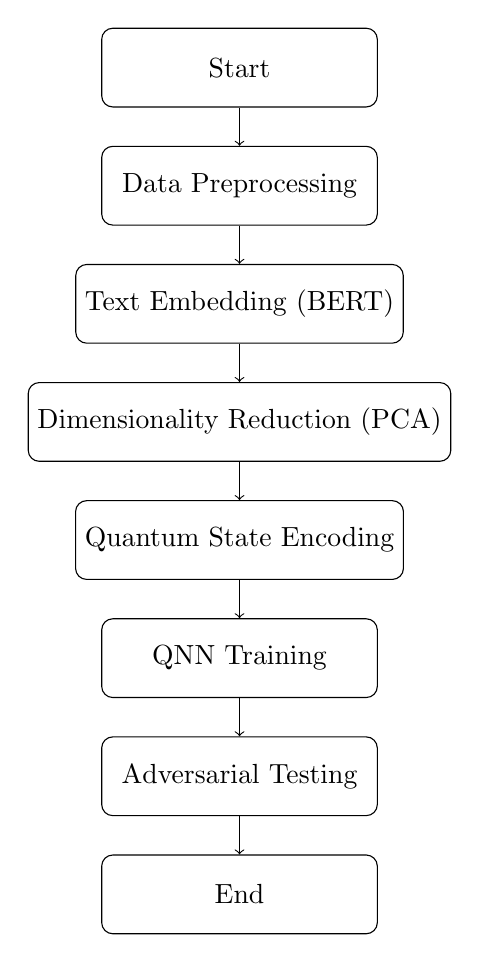
\begin{tikzpicture}[node distance=1.5cm, every node/.style={rectangle, draw, rounded corners, align=center, minimum width=3.5cm, minimum height=1cm}]
\node (start) {Start};
\node (prep) [below of=start] {Data Preprocessing};
\node (embed) [below of=prep] {Text Embedding (BERT)};
\node (reduce) [below of=embed] {Dimensionality Reduction (PCA)};
\node (encode) [below of=reduce] {Quantum State Encoding};
\node (qnn) [below of=encode] {QNN Training};
\node (adv) [below of=qnn] {Adversarial Testing};
\node (end) [below of=adv] {End};

\draw[->] (start) -- (prep);
\draw[->] (prep) -- (embed);
\draw[->] (embed) -- (reduce);
\draw[->] (reduce) -- (encode);
\draw[->] (encode) -- (qnn);
\draw[->] (qnn) -- (adv);
\draw[->] (adv) -- (end);
\end{tikzpicture}
\caption{Overview of the proposed methodology.}
\label{fig:flowchart}
\end{figure}
